\section{Bidirectional Similarity}
As we have seen in the first section that resizing and croping do no not fit our estimations of a smaller representation. This section will introduce an algorithm called 'bidirectional similarity' found by \textsc{Simakov, Caspi, Shechtman} and \textsc{Irani}.\\
It works by gradually resizing the original image and recalculate then the pixels by comparing target image with orignal image for completeness and coherence.\\
The next subsections will explain every step of the algorithm by detail, beginning with the terms 'complete' and 'coherent'.

\subsection{Completeness and Coherence}
\begin{figure}[h]
\centering
\includegraphics[scale=0.6]{img/cac}
\caption[Completeness and Coherence]{A basic example for completeness and coherence. Target image \textit{T\textsubscript{1}} satisifies completeness, \textit{T\textsubscript{2}} is coherent and \textit{T\textsubscript{3}} fulfills both - completeness and coherence.}
\label{fig:Completeness and Coherence}
\end{figure}

Completeness and Coherence are terms to describe similarity between two related images. Figure \ref{fig:Completeness and Coherence} shows a basic example, where the source image contains two colored areas - a green and a red one. A target image is called 'complete' when it contains all visual informations of the source image. \textit{T\textsubscript{1}} is therefore complete, because it contains both colored areas of the source image \textit{S}, additionally it contains a purple star.\\
On the other hand an image is called 'coherent' when it does not introduce new visual artifacts, which the source image does not contain. Target image \textit{T\textsubscript{2}} is coherent, because it has no new visual informations in it, but it lacks the red area.\\
If a target image satisfies both criteria - like \textit{T\textsubscript{3}} does - then it is complete and coherent. So \textit{T\textsubscript{3}} is more similar to \textit{S} than \textit{T\textsubscript{1}} and \textit{T\textsubscript{2}}.\\
Now knowing what those terms describe it is important to take a look on how they work technically.

\subsubsection*{Completeness}
\begin{figure}[h]
\centering
\includegraphics[scale=0.65]{img/completeness}
\caption[Completenesse]{Schematic example for completeness check.}
\label{fig:Completeness}
\end{figure}

As discussed before completeness describes that the target image contains every information of the source image. Figure \ref{fig:Completeness} shows how this works technically. For every patch \textit{P} in source image \textit{S} compare it with every possible patch in \textit{T} and find the most similar to it.

\subsubsection*{Coherence}
\begin{figure}[h]
\centering
\includegraphics[scale=0.65]{img/coherence}
\caption[Coherence]{Schematic example for coherence check.}
\label{fig:Coherence}
\end{figure}

Checking for coherence works similar to completeness except the direction of comparison has changed. Figure \ref{fig:Coherence} shows it. Now for every patch \textit{Q} in \textit{T} compare it with every possible patch in \textit{S} and find the most similar to it.\\
Note that it is not enough to check in only one direction because the algorithm could miss to find for example new artifacts which the completeness check does not find.\\
In other words: \textit{Q} can be the most similar patch to \textit{P}, but \textit{P} does not have to be the most similar patch to \textit{Q}.

\subsubsection*{Examples}
\begin{figure}[h]
\centering
\includegraphics[scale=0.9]{img/compcohexample}
\caption[Compcohexample]{Completeness and coherence examples with real photos. The upper image shows some buildings with persons in front and three variants of target images.\\ The lower photo shows a person and a animal with three variants of target images.\\ Additionally there are shown the distance values introduced in section 2.2.\\ Examples from \cite{bisi} }
\label{fig:Compcohexample}
\end{figure}

Figure \ref{fig:Compcohexample} shows some examples for completeness and coherence with real photos. The complete images show every informations of the source images like buildings, persons and the animal but there are also some seams which are not in the source image.\\
The coherent images which where achieved by croping \cite{bisi} do not have any seams or other new artifacts but they miss the persons on them.\\
The complete and coherent target images do have all information like buildings, persons and animal, and they do not introduce new artifacts. They are results of the bidrectional similarity summarization \cite{bisi}.


\subsection{Measurement}
Before taking a step further to the algorithm it is important to know how to measure bidirectional similarity between a source image and a target image. From the previous subsection 2.1 we know how completeness and coherence work technically. The remaining step now is to convert it to a mathematical equation as described in \cite{bisi}.

\subsubsection*{Measure completeness}
For every patch \textit{P} in \textit{S} compare it to every possible patch \textit{Q} in \textit{T} and find one with minimal difference. (Fig. \ref{fig:Completeness})

\large
\begin{equation}
\label{Eq:Measure completeness}
d_{complete}(S,T)=\frac{1}{N_{S}}\sum_{P \subset S} \min\limits_{Q \subset T} D(P,Q)
\end{equation}
\normalsize

Eq. \ref{Eq:Measure completeness} calculates the \textit{distance d} between source image \textit{S} and target image \textit{T} in relation to completeness. \textit{N\textsubscript{S}} is the number of patches in \textit{S} for weighted average of the distance.

\subsubsection*{Measure coherence}
For every patch \textit{Q} in \textit{T} compare it to every possible patch \textit{P} in \textit{S} and find one with minimal difference. (Fig. \ref{fig:Coherence})

\large
\begin{equation}
\label{Eq:Measure coherence}
d_{cohere}(S,T)=\frac{1}{N_{T}}\sum_{Q \subset T} \min\limits_{P \subset S} D(Q,P)
\end{equation}
\normalsize

Like for completeness measure Eq. \ref{Eq:Measure coherence} calculates \textit{d} in relation to coherence. \textit{N\textsubscript{T}} is the number of patches in \textit{T} for weighted average of the distance.

\subsubsection*{Overall distance and examples}
To calculate the overall distance we just add \textit{d\textsubscript{cohere}} to \textit{d\textsubscript{complete}}.

\large
\begin{align}
\label{Eq:Overall measure}
d(S,T)&=d_{complete}(S,T)+d_{cohere}(S,T) \nonumber \\
&=\frac{1}{N_{S}}\sum_{P \subset S} \min\limits_{Q \subset T} D(P,Q)+\frac{1}{N_{T}}\sum_{Q \subset T} \min\limits_{P \subset S} D(Q,P)
\end{align}
\normalsize

Figure \ref{fig:Compcohexample} on page \pageref{fig:Compcohexample} shows distance values by Eq. \ref{Eq:Overall measure} for some target images. The worst values are found for complete images, the best for complete and coherent images. A value of 0 means that the images are the same.

\subsection{Algorithm}
With all the knowledge it is now possible to introduce the algorithm. First of all the goal of the algorithm is to minimize Eq. \ref{Eq:Overall measure}:

\large
\begin{equation}
\label{Eq:Minimize distance}
T_{output}=\text{arg} \min\limits_{T}d(S,T)
\end{equation}
\normalsize

\subsubsection{Gradual resizing}
As mentioned in the beginning of this section the algorithm uses \textit{gradual resizing}. This means that in every step the next target image will be shrinked a little bit and the pixels are then recalculated.\\
The critical step is to find a good initial guess for shrinking the image. If the shrinking amount is to big some valueable information could get lost because of quality reduction. So \cite{bisi} found out that shrinking to a size of 95\% supplies good results.\\
Figure \ref{fig:Gradual resizing} shows an example for gradual resizing. As it can be clearly seen every step has its own output image \textit{T\textsubscript{k}} and the most possible minimal distance value for its size.

\begin{figure}[h]
\centering
\includegraphics[scale=0.8]{img/gradualresizing}
\caption[Gradual resizing]{The upper images show an example of gradual resizing. The lower image describes the algorithm with gradual resizing and using the update rule introduced in subsection 2.3.2.\\ Images by \cite{bisi}. }
\label{fig:Gradual resizing}
\end{figure}

\subsubsection{Update rule}
After every resizing step the pixels must be recalculated to maintain the quality of the orignal image. This is done by the \textit{update rule}.

\begin{figure}[h]
\centering
\includegraphics[scale=0.7]{img/updaterule}
\caption[Update rule]{This figure shows how the update rule votes the color for one pixel \textit{q} in the target image \textit{T}.}
\label{fig:Update rule}
\end{figure}

The update rule as desrcibed in \cite{bisi}:

\vspace{15px}
1. For each patch $\hat{P} \subset S$ find most similar patch $\hat{Q} \subset T^{(l)}$. Pixels in $\hat{P}$ vote for pixels in $\hat{Q}$ with weight $\frac{1}{N_{S}}$. (Completeness)

\vspace{15px}
2. For each patch $Q \subset T^{(l)}$ find the most similar source patch $P \subset S$. Colors of pixels in \textit{P} are votes for pixel in \textit{Q} with weight $\frac{1}{N_{T}}$. (Coherence)

\vspace{15px}
3. For each target pixel $q$ take weighted average of all its votes as its new color $T^{(l+1)}(q)$.

\vspace{15px}
With those steps we receive following equation for the update rule:
\large
\begin{equation}
\label{Eq:Update rule}
T(q)=\frac{\frac{1}{N_{S}} \sum_{j=1}^{n} S(\hat{p}_{j}) + \frac{1}{N_{T}} \sum_{i=1}^{m} S(p_{i})}{\frac{n}{N_{S}} + \frac{m}{N_{T}}}
\end{equation}
\normalsize

\subsubsection{Importance weights}
\subsection{Performance and limitations}